\documentclass{article}

% NeurIPS 2020 style
\usepackage[final,nonatbib]{neurips_2020}

% Packages
\usepackage[utf8]{inputenc}
\usepackage[T1]{fontenc}
\usepackage{hyperref}
\usepackage{url}
\usepackage{booktabs}
\usepackage{amsfonts}
\usepackage{amsmath}
\usepackage{amssymb}
\usepackage{nicefrac}
\usepackage{microtype}
\usepackage{xcolor}
\usepackage{graphicx}
\usepackage{algorithm}
\usepackage{algorithmic}
\usepackage{tikz}
\usepackage{multirow}
\usetikzlibrary{shapes.geometric,arrows.meta,positioning,fit,backgrounds}

% Custom commands
\newcommand{\threatforest}{\textsc{ThreatForest}}
\newcommand{\todo}[1]{\textcolor{red}{\textbf{[TODO: #1]}}}

\title{\threatforest{}: Multi-Agent Attack Tree Generation\\with MITRE ATT\&CK Mapping}

\author{
  Cristian Leo \\
  Amazon Web Services \\
  \texttt{crisleoo@amazon.com} \\
  \And
  Anton Dykyi \\
  Amazon Web Services \\
  \texttt{antondk@amazon.co.uk} \\
  \And
  Danny Cortegaca \\
  Amazon Web Services \\
  \texttt{dicorteg@amazon.co.uk} \\
  \And
  Daniel Begimher \\
  Amazon Web Services \\
  \texttt{dbbegimh@amazon.com} \\
}

\begin{document}

\maketitle

\begin{abstract}
Threat modeling is essential for secure software development, yet manual analysis of cloud-native architectures is time-consuming and requires scarce security expertise. We present \threatforest{}, a multi-agent system that automatically generates structured attack trees from source code repositories, maps attack steps to MITRE ATT\&CK techniques, and synthesizes actionable mitigations. \threatforest{} decomposes threat modeling into a six-stage pipeline---repository analysis, threat generation, attack tree construction, TTP mapping, mitigation synthesis, and report generation---orchestrated as a directed graph with deterministic verification gates. A key technical contribution is our hybrid TTP mapping approach: domain-specific embeddings (ATTACK-BERT) retrieve candidate techniques via cosine similarity, followed by an LLM reviewer that refines mappings with access to top-$K$ alternatives. We evaluate \threatforest{} across \todo{N} application domains using 16 scoring dimensions spanning four capabilities, supported by an observability infrastructure built on OpenTelemetry and Langfuse that enables both automated metrics and subject matter expert (SME) review. \todo{Baseline results summary.} To our knowledge, \threatforest{} is the first end-to-end system that takes a code repository as input and produces MITRE ATT\&CK-mapped attack trees with evidence-based mitigations.
\end{abstract}

%==============================================================================
\section{Introduction}
%==============================================================================

Threat modeling is a cornerstone of secure software development~\cite{shostack2014threat}, requiring practitioners to systematically identify threats, analyze attack vectors, and propose mitigations. As cloud-native architectures grow in complexity, manual threat modeling becomes increasingly impractical---a single system may expose hundreds of attack surfaces across multiple services, each requiring domain-specific security expertise.

Large language models (LLMs) offer a path toward automating this process. Recent multi-agent systems can generate threat statements, construct attack trees~\cite{schneier1999attack}, and map findings to frameworks like MITRE ATT\&CK~\cite{strom2018mitre}. However, a fundamental question remains unanswered: \emph{how do we measure whether automated threat models are any good?}

Unlike code generation---where correctness can be verified by compilation and test suites---threat modeling quality is inherently multi-dimensional and subjective. A generated attack tree may be syntactically valid yet unrealistic, structurally complete yet missing critical attack phases, or technically accurate yet unhelpful for defenders. No existing benchmark or evaluation methodology addresses this challenge.

We identify three gaps in the current landscape:

\textbf{No standardized evaluation dimensions.} Existing work evaluates threat modeling tools informally, typically through case studies or user surveys. There is no agreed-upon set of quality dimensions, scoring scales, or evaluation protocols.

\textbf{No separation of capabilities.} Automated threat modeling involves distinct sub-tasks---generating threat statements, constructing attack trees, mapping to TTP frameworks---each requiring different evaluation criteria. Existing approaches conflate these into a single quality judgment.

\textbf{No infrastructure for iterative improvement.} Without structured data collection and scoring, there is no path from evaluation to optimization. Improving prompt quality requires ground truth datasets that do not yet exist.

We address these gaps with an evaluation framework for \threatforest{}, a multi-agent threat modeling system. Our contributions are:

\begin{enumerate}
    \item \textbf{Multi-dimensional evaluation taxonomy.} We decompose threat modeling quality into three capabilities---threat statement generation, attack tree generation, and TTP matching---with 12 score dimensions across a standardized 5-point categorical scale.

    \item \textbf{Hybrid evaluation methodology.} We combine automated structural metrics (node count, path coverage, phase detection, syntax validation) with SME scoring protocols, enabling both scalable measurement and expert validation.

    \item \textbf{Tracing infrastructure.} We implement the framework as a production tracing system built on OpenTelemetry and Langfuse, capturing every agent interaction with structured metadata, scores, and export pipelines for dataset curation.

    \item \textbf{Baseline measurements.} We report the first quantitative baselines for automated threat modeling quality across \todo{N} diverse domains.

    \item \textbf{Optimization roadmap.} We describe how the evaluation framework enables iterative prompt optimization via DSPy's MIPROv2~\cite{opsahlong2024miprov2}, where SME-scored traces feed directly into reflective optimization cycles.
\end{enumerate}

%==============================================================================
\section{Related Work}
%==============================================================================

\textbf{Threat modeling methodologies.}
STRIDE~\cite{shostack2014threat} categorizes threats into six classes (Spoofing, Tampering, Repudiation, Information Disclosure, Denial of Service, Elevation of Privilege) and remains the most widely adopted methodology. Attack trees~\cite{schneier1999attack} model adversary goals as hierarchical decompositions with AND/OR nodes, enabling quantitative risk analysis. PASTA (Process for Attack Simulation and Threat Analysis) adds a risk-centric perspective. These methodologies provide structure but require manual expertise for every system analyzed.

\textbf{Tool-assisted threat modeling.}
Microsoft Threat Modeling Tool~\cite{microsoft-tmt} generates STRIDE-based threats from data flow diagrams but requires manual diagram construction. OWASP Threat Dragon~\cite{owasp-threatdragon} offers open-source diagramming with threat rule engines. AWS Threat Composer~\cite{aws-threatcomposer} provides guided threat statement authoring with structured templates. None of these tools automate the reasoning required to generate attack trees or map threats to standardized frameworks.

\textbf{LLM-based threat analysis.}
ThreatModeling-LLM~\cite{threatmodeling-llm2024} automates threat identification for banking systems through dataset creation, prompt engineering, and model fine-tuning, achieving promising results on domain-specific threats. Bhatia et al.~\cite{canllmsthreatmodel2025} evaluate whether LLMs can threat model real-world cloud infrastructure, finding that GPT-4.1 and Gemini 2.5 Pro excel at threat identification but with varying performance across prompting strategies. ThreatLens uses retrieval-augmented generation for hardware security verification. These approaches focus on threat \emph{identification} but do not produce structured attack trees or TTP mappings.

\textbf{MITRE ATT\&CK mapping.}
Automated mapping of security text to ATT\&CK techniques has been approached through NLP classification. CVE2ATT\&CK~\cite{cve2attack2022} uses BERT-based models to map CVE descriptions to ATT\&CK techniques. SMET~\cite{smet2023} trains ATT\&CK BERT using a Siamese network to learn semantic similarity among attack actions, achieving state-of-the-art results on CVE-to-technique mapping. Kim et al.~\cite{modernbert2025} combine ModernBERT with BERTopic for tactic-level classification. These works map \emph{existing} vulnerability descriptions to techniques; \threatforest{} maps \emph{generated} attack tree steps---a distinct task requiring the model to bridge the gap between abstract attack descriptions and concrete ATT\&CK techniques.

\textbf{Domain-specific language models for cybersecurity.}
SecureBERT~\cite{aghaei2023securebert} adapts BERT to cybersecurity text, improving performance on NER and classification tasks. ATTACK-BERT~\cite{attackbert} extends sentence-transformers to produce embeddings specifically for attack action descriptions, enabling semantic similarity search against ATT\&CK technique descriptions. We leverage ATTACK-BERT as the retrieval component in our hybrid TTP mapping pipeline (\S\ref{sec:ttp}).

\textbf{Multi-agent systems.}
The Strands Agents SDK~\cite{strands2025} provides a graph-based orchestration framework for multi-agent workflows with tool use, streaming, and telemetry. While multi-agent architectures have been applied to code generation, software testing, and general reasoning, their application to security threat modeling---where outputs must be both technically accurate and structurally valid---remains unexplored.

%==============================================================================
\section{System Architecture}
\label{sec:architecture}
%==============================================================================

\threatforest{} decomposes threat modeling into six stages, each implemented as an autonomous agent with tool access, orchestrated as a directed graph with verification gates. Figure~\ref{fig:pipeline} shows the full pipeline.

\begin{figure}[t]
\centering
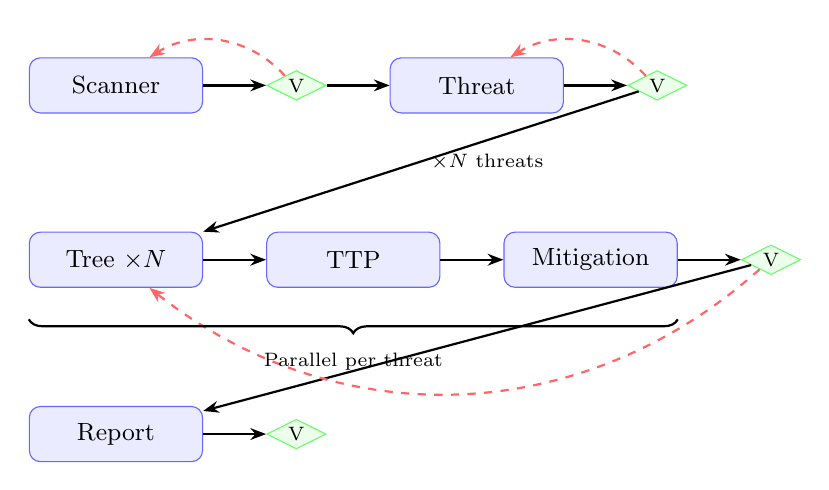
\begin{tikzpicture}[
    node distance=1.2cm and 0.8cm,
    agent/.style={rectangle, draw=blue!60, fill=blue!8, rounded corners, minimum width=2.2cm, minimum height=0.7cm, font=\small},
    verifier/.style={diamond, draw=green!60, fill=green!8, aspect=2, font=\scriptsize, inner sep=1pt},
    arrow/.style={-{Stealth[length=2mm]}, thick},
    retry/.style={-{Stealth[length=2mm]}, thick, dashed, red!60},
]
    \node[agent] (scanner) {Scanner};
    \node[verifier, right=of scanner] (sv) {V};
    \node[agent, right=of sv] (threat) {Threat};
    \node[verifier, right=of threat] (tv) {V};
    \node[agent, below=1.5cm of scanner] (tree) {Tree $\times N$};
    \node[agent, right=of tree] (ttp) {TTP};
    \node[agent, right=of ttp] (mit) {Mitigation};
    \node[verifier, right=of mit] (pv) {V};
    \node[agent, below=1.5cm of tree] (report) {Report};
    \node[verifier, right=of report] (rv) {V};

    \draw[arrow] (scanner) -- (sv);
    \draw[arrow] (sv) -- (threat);
    \draw[arrow] (threat) -- (tv);
    \draw[arrow] (tv) -- node[right, font=\scriptsize] {$\times N$ threats} (tree);
    \draw[arrow] (tree) -- (ttp);
    \draw[arrow] (ttp) -- (mit);
    \draw[arrow] (mit) -- (pv);
    \draw[arrow] (pv) -- (report);
    \draw[arrow] (report) -- (rv);

    \draw[retry] (sv) to[bend right=40] (scanner);
    \draw[retry] (tv) to[bend right=40] (threat);
    \draw[retry] (pv) to[bend left=40] (tree);

    % Parallel bracket
    \draw[decorate, decoration={brace, amplitude=5pt, mirror}, thick] ([yshift=-0.4cm]tree.south west) -- ([yshift=-0.4cm]mit.south east) node[midway, below=0.3cm, font=\scriptsize] {Parallel per threat};
\end{tikzpicture}
\caption{The \threatforest{} pipeline. Boxes are LLM agents; diamonds are deterministic verifiers. Dashed arrows indicate retry edges on verification failure. The tree$\to$TTP$\to$mitigation sub-pipeline runs in parallel for each threat.}
\label{fig:pipeline}
\end{figure}

%----------------------------------------------------------------------
\subsection{Pipeline Overview and Graph Orchestration}
\label{sec:orchestration}
%----------------------------------------------------------------------

The pipeline is implemented as a Strands Graph~\cite{strands2025}---a directed graph where nodes are agent executors and edges carry conditional predicates. Each agent reads its predecessor's output from a shared state directory (\texttt{.threatforest/state/}) and writes structured JSON. This file-based state passing provides three benefits: (1) intermediate outputs are inspectable for debugging, (2) the pipeline is resumable after failures, and (3) parallel agents avoid shared-memory concurrency issues.

The graph defines retry edges: when a verifier detects invalid output, execution flows back to the producing agent for a second attempt, up to a configurable budget of 50 total node executions. This provides self-healing behavior without requiring explicit error handling in each agent.

%----------------------------------------------------------------------
\subsection{Scanner and Threat Generation}
\label{sec:scanner-threat}
%----------------------------------------------------------------------

\textbf{Scanner Agent.} The scanner receives a repository path and uses two tools: a \emph{structural analyzer} that extracts the project's file tree, dependency manifests, and infrastructure-as-code definitions; and a \emph{sandboxed file reader} restricted to the repository directory. The agent produces a \emph{project context} containing: cloud provider, technology stack, services, authentication mechanisms, data flows, and deployment model. A deterministic verifier checks that all required fields are present and non-empty.

\textbf{Threat Agent.} The threat agent receives the project context and generates structured threat statements following the pattern:

\begin{quote}
\emph{A [actor] with [access/knowledge], can [action], which leads to [impact], resulting in [consequence].}
\end{quote}

Each threat includes a title, description, priority, and affected components. The verifier validates JSON structure and ensures each threat references components identified in the scanner context.

%----------------------------------------------------------------------
\subsection{Attack Tree Generation}
\label{sec:tree}
%----------------------------------------------------------------------

Attack trees are generated in parallel: one sub-pipeline per threat, all executing concurrently. Each tree agent receives the scanner context and a single threat, producing a hierarchical attack tree where:

\begin{itemize}
    \item The \textbf{root node} represents the adversary's goal (derived from the threat statement).
    \item \textbf{Intermediate nodes} decompose the goal into sub-goals with AND/OR relationships.
    \item \textbf{Leaf nodes} represent concrete attack techniques.
\end{itemize}

Each step $s_i$ in the tree is a tuple $(id, title, description, parent\_id, is\_leaf, category)$ where $category \in \{\text{fact}, \text{action}, \text{detection}, \text{gate}\}$. The tree structure enables systematic enumeration of attack paths: each root-to-leaf path represents a complete attack scenario.

For a system with $N$ threats, the parallel fan-out produces $N$ independent sub-pipelines (tree $\to$ TTP $\to$ mitigation), providing approximately $N\times$ speedup over sequential execution.

%----------------------------------------------------------------------
\subsection{TTP Mapping: Hybrid Embedding + LLM}
\label{sec:ttp}
%----------------------------------------------------------------------

Mapping attack tree steps to MITRE ATT\&CK techniques is the most technically challenging stage. We employ a two-phase hybrid approach that combines the efficiency of embedding-based retrieval with the contextual reasoning of an LLM.

\textbf{Phase 1: Embedding Retrieval.}
Each attack step description $d_i$ is encoded using ATTACK-BERT~\cite{attackbert}, a sentence-transformer fine-tuned on cybersecurity text. We compute cosine similarity against pre-encoded ATT\&CK technique descriptions $\{t_1, \ldots, t_M\}$ where $M$ is the number of techniques in the ATT\&CK matrix:

\begin{equation}
\text{sim}(d_i, t_j) = \frac{\mathbf{e}(d_i) \cdot \mathbf{e}(t_j)}{\|\mathbf{e}(d_i)\| \, \|\mathbf{e}(t_j)\|}
\label{eq:cosine}
\end{equation}

where $\mathbf{e}(\cdot)$ denotes the ATTACK-BERT embedding function. For each step $d_i$, we retrieve the top-$K$ candidates ranked by similarity:

\begin{equation}
\text{candidates}(d_i) = \text{top-}K\left(\{\text{sim}(d_i, t_j) \mid j = 1, \ldots, M\}\right)
\label{eq:topk}
\end{equation}

We use $K=5$ and a minimum similarity threshold $\tau = 0.3$. The top-1 candidate is selected as the initial mapping.

\textbf{Phase 2: LLM Reviewer.}
The embedding-based top-1 mapping is often correct for well-described attack steps but fails when surface-level textual similarity diverges from semantic intent. For example, a step describing ``credential theft via compromised IAM role'' may match ``T1557.004 Evil Twin'' (a Wi-Fi attack) based on shared vocabulary around ``compromise'' rather than the semantically correct ``T1078.004 Valid Accounts: Cloud Accounts.''

The LLM reviewer agent receives the top-1 summary and has access to a \texttt{get\_ttp\_alternatives} tool that returns the full top-$K$ candidates for any step. The reviewer:
\begin{enumerate}
    \item Examines each top-1 mapping for semantic correctness.
    \item For suspicious mappings, queries alternatives and selects the best match.
    \item Records whether it overrode the embedding's top-1 and provides reasoning.
\end{enumerate}

This hybrid approach leverages the embedding model's efficiency (encoding all steps in a single batch) while using the LLM only for refinement, keeping costs proportional to the number of overrides rather than the total number of steps.

%----------------------------------------------------------------------
\subsection{Mitigation and Verification}
\label{sec:mitigation}
%----------------------------------------------------------------------

\textbf{Mitigation Agent.} The mitigation agent receives the attack trees, TTP mappings, and scanner context, synthesizing per-technique mitigations. Each mitigation includes: the specific AWS service or configuration to implement, the attack steps it addresses, and evidence linking the mitigation to the identified technique. This evidence-based approach ensures mitigations are actionable rather than generic.

\textbf{Verifier Pattern.} Every stage in the pipeline includes a deterministic verifier---a pure function (no LLM) that validates structural properties of the output:

\begin{itemize}
    \item \textbf{Scanner verifier}: All required context fields present and non-empty.
    \item \textbf{Threat verifier}: Valid JSON, each threat has required fields, references valid components.
    \item \textbf{Pipeline verifier}: Attack trees have valid parent-child relationships, TTP mappings reference existing steps, mitigations reference existing techniques.
    \item \textbf{Report verifier}: Output file exists with expected sections.
\end{itemize}

On verification failure, the graph's retry edge routes execution back to the producing agent. This pattern provides quality gates without the cost or non-determinism of LLM-based validation.

\textbf{Report Generator.} The final stage is deterministic (no LLM): it compiles all state files into a structured Markdown report and an interactive HTML dashboard with attack tree visualizations.

%==============================================================================
\section{Evaluation Methodology}
\label{sec:evaluation}
%==============================================================================

We design an evaluation framework that combines automated structural metrics with human expert assessment, supported by an observability infrastructure that captures every agent interaction.

%----------------------------------------------------------------------
\subsection{Scoring Dimensions}
%----------------------------------------------------------------------

We define 16 scoring dimensions across four capabilities, each using a 5-point categorical scale $\mathcal{C} = \{\text{excellent}, \text{good}, \text{acceptable}, \text{poor}, \text{unacceptable}\}$ mapped to numeric values $\{1.0, 0.75, 0.5, 0.25, 0.0\}$:

\textbf{Threat Statement Quality} (5 dimensions): overall quality, relevance to application context, completeness of threat coverage, technical accuracy, and hallucination detection.

\textbf{Attack Tree Quality} (6 dimensions): overall quality, structural quality (depth, branching, organization), technical realism of attack techniques, logical progression of attack paths, completeness of attack vector coverage, and actionability for defenders.

\textbf{TTP Mapping Quality} (1 dimension): correctness of MITRE ATT\&CK technique assignment, using a specialized scale replacing ``unacceptable'' with ``no\_mapping'' for steps where no technique applies.

\textbf{Mitigation Quality} (4 dimensions): actionability (concrete implementable steps), specificity to the identified threat and technology stack, coverage of identified attack paths, and technical accuracy of recommended controls.

%----------------------------------------------------------------------
\subsection{Observability Infrastructure}
%----------------------------------------------------------------------

\threatforest{} produces two complementary trace types:

\textbf{OTEL traces} (automatic). The Strands SDK~\cite{strands2025} emits OpenTelemetry spans for every LLM call, tool invocation, and agent event loop cycle. These are exported to Langfuse~\cite{langfuse2024} via the OTLP protocol, capturing token counts, latencies, model parameters, and full input/output content. All traces within a pipeline run share a session identifier for grouping.

\textbf{Annotation traces} (structured). At each subgraph boundary (scanner, threat generation, attack tree generation, TTP mapping, mitigation generation), we push a Langfuse SDK trace with clean input/output JSON. These traces are tagged with \texttt{annotation} for routing to SME review queues.

%----------------------------------------------------------------------
\subsection{SME Review Pipeline}
%----------------------------------------------------------------------

Annotation traces are routed to Langfuse annotation queues---one per capability. Each queue presents the reviewer with the agent's input context and generated output, along with the applicable scoring dimensions. Reviewers assign categorical scores independently for each dimension and may add free-text feedback.

%----------------------------------------------------------------------
\subsection{TTP Ground Truth Dataset}
%----------------------------------------------------------------------

Individual TTP mappings are automatically pushed as Langfuse dataset items with the attack step description as input and the mapped technique as metadata. The \texttt{expected\_output} field is initially null; SMEs label each mapping as correct or incorrect, building a ground truth corpus over time. This corpus serves dual purposes: (1) evaluating embedding retrieval accuracy via precision@$K$, and (2) providing training pairs for fine-tuning domain-specific embedding models.

%----------------------------------------------------------------------
\subsection{Automated Structural Metrics}
%----------------------------------------------------------------------

We compute the following metrics automatically from pipeline outputs:

\begin{itemize}
    \item \textbf{Tree depth}: Maximum root-to-leaf path length per attack tree.
    \item \textbf{Step count}: Total attack steps across all trees.
    \item \textbf{Technique diversity}: $|\text{unique techniques}| / |\text{total mappings}|$, measuring how broadly the system maps across ATT\&CK.
    \item \textbf{Phase coverage}: Fraction of ATT\&CK tactics (Initial Access through Impact) represented in the generated mappings.
    \item \textbf{Reviewer override rate}: Fraction of TTP mappings where the LLM reviewer changed the embedding's top-1 selection.
\end{itemize}

%==============================================================================
\section{Results}
\label{sec:results}
%==============================================================================

We evaluate \threatforest{} on \todo{N} sample applications spanning diverse cloud architectures. All experiments use Claude Opus 4.6 via AWS Bedrock with ATTACK-BERT for TTP embedding retrieval.

%----------------------------------------------------------------------
\subsection{Pipeline Output Summary}
%----------------------------------------------------------------------

Table~\ref{tab:pipeline-summary} summarizes the pipeline outputs across domains.

\begin{table}[t]
\centering
\caption{Pipeline output summary across application domains.}
\label{tab:pipeline-summary}
\begin{tabular}{lrrrrrr}
\toprule
\textbf{Domain} & \textbf{Threats} & \textbf{Trees} & \textbf{Steps} & \textbf{TTPs} & \textbf{Unique} & \textbf{Mitigations} \\
\midrule
S3 Multi-Tenant SaaS & \todo{} & \todo{} & \todo{} & \todo{} & \todo{} & \todo{} \\
Healthcare (HCLS) & \todo{} & \todo{} & \todo{} & \todo{} & \todo{} & \todo{} \\
IoT Device Mgmt & \todo{} & \todo{} & \todo{} & \todo{} & \todo{} & \todo{} \\
Vehicle Platform & \todo{} & \todo{} & \todo{} & \todo{} & \todo{} & \todo{} \\
\todo{More domains} & & & & & & \\
\midrule
\textbf{Average} & \todo{} & \todo{} & \todo{} & \todo{} & \todo{} & \todo{} \\
\bottomrule
\end{tabular}
\end{table}

%----------------------------------------------------------------------
\subsection{Structural Quality Metrics}
%----------------------------------------------------------------------

Table~\ref{tab:structural} reports automated structural metrics.

\begin{table}[t]
\centering
\caption{Structural quality metrics across domains.}
\label{tab:structural}
\begin{tabular}{lrrrr}
\toprule
\textbf{Domain} & \textbf{Avg Depth} & \textbf{Avg Steps/Tree} & \textbf{Technique Diversity} & \textbf{Phase Coverage} \\
\midrule
S3 Multi-Tenant SaaS & \todo{} & \todo{} & \todo{} & \todo{} \\
Healthcare (HCLS) & \todo{} & \todo{} & \todo{} & \todo{} \\
IoT Device Mgmt & \todo{} & \todo{} & \todo{} & \todo{} \\
Vehicle Platform & \todo{} & \todo{} & \todo{} & \todo{} \\
\midrule
\textbf{Average} & \todo{} & \todo{} & \todo{} & \todo{} \\
\bottomrule
\end{tabular}
\end{table}

%----------------------------------------------------------------------
\subsection{TTP Mapping Analysis}
%----------------------------------------------------------------------

Table~\ref{tab:ttp} analyzes the hybrid TTP mapping approach.

\begin{table}[t]
\centering
\caption{TTP mapping analysis. Embedding accuracy is top-1 precision before LLM review; post-review accuracy is measured against SME labels.}
\label{tab:ttp}
\begin{tabular}{lrrrr}
\toprule
\textbf{Domain} & \textbf{Total Mappings} & \textbf{Override Rate} & \textbf{Embedding Acc.} & \textbf{Post-Review Acc.} \\
\midrule
S3 Multi-Tenant SaaS & \todo{} & \todo{} & \todo{} & \todo{} \\
Healthcare (HCLS) & \todo{} & \todo{} & \todo{} & \todo{} \\
IoT Device Mgmt & \todo{} & \todo{} & \todo{} & \todo{} \\
Vehicle Platform & \todo{} & \todo{} & \todo{} & \todo{} \\
\midrule
\textbf{Average} & \todo{} & \todo{} & \todo{} & \todo{} \\
\bottomrule
\end{tabular}
\end{table}

The override rate measures how often the LLM reviewer changed the embedding's top-1 selection. A high override rate indicates the embedding model struggles with the domain; a low rate with high post-review accuracy suggests the embedding is reliable and the reviewer adds marginal value.

%----------------------------------------------------------------------
\subsection{SME Evaluation Scores}
%----------------------------------------------------------------------

\todo{Table with SME scores per dimension, per domain. Median and IQR across reviewers. Include inter-rater reliability (Cohen's $\kappa$ or Krippendorff's $\alpha$).}

\begin{table}[t]
\centering
\caption{SME evaluation scores (median) across domains. Scale: 1.0 = Excellent, 0.0 = Unacceptable.}
\label{tab:sme-scores}
\begin{tabular}{lrrrr}
\toprule
\textbf{Dimension} & \textbf{S3} & \textbf{HCLS} & \textbf{IoT} & \textbf{Vehicle} \\
\midrule
\multicolumn{5}{l}{\emph{Threat Statements}} \\
\quad Overall Quality & \todo{} & \todo{} & \todo{} & \todo{} \\
\quad Relevance & \todo{} & \todo{} & \todo{} & \todo{} \\
\quad Completeness & \todo{} & \todo{} & \todo{} & \todo{} \\
\quad Technical Accuracy & \todo{} & \todo{} & \todo{} & \todo{} \\
\quad Hallucination & \todo{} & \todo{} & \todo{} & \todo{} \\
\midrule
\multicolumn{5}{l}{\emph{Attack Trees}} \\
\quad Overall Quality & \todo{} & \todo{} & \todo{} & \todo{} \\
\quad Structural Quality & \todo{} & \todo{} & \todo{} & \todo{} \\
\quad Technical Realism & \todo{} & \todo{} & \todo{} & \todo{} \\
\quad Attack Path Logic & \todo{} & \todo{} & \todo{} & \todo{} \\
\quad Completeness & \todo{} & \todo{} & \todo{} & \todo{} \\
\quad Actionability & \todo{} & \todo{} & \todo{} & \todo{} \\
\midrule
\multicolumn{5}{l}{\emph{TTP Mapping}} \\
\quad Mapping Quality & \todo{} & \todo{} & \todo{} & \todo{} \\
\midrule
\multicolumn{5}{l}{\emph{Mitigations}} \\
\quad Actionability & \todo{} & \todo{} & \todo{} & \todo{} \\
\quad Specificity & \todo{} & \todo{} & \todo{} & \todo{} \\
\quad Coverage & \todo{} & \todo{} & \todo{} & \todo{} \\
\quad Technical Accuracy & \todo{} & \todo{} & \todo{} & \todo{} \\
\bottomrule
\end{tabular}
\end{table}

%==============================================================================
\section{Discussion}
%==============================================================================

\subsection{Framework Design Decisions}

\textbf{Categorical vs.\ numeric scales.} We chose a 5-point categorical scale over continuous numeric scores to reduce SME cognitive load and improve inter-rater reliability. Categorical labels (``excellent'' through ``unacceptable'') provide clearer anchoring than arbitrary numeric ranges, while the fixed mapping to $[0, 1]$ preserves compatibility with optimization objectives.

\textbf{Production tracing vs.\ offline evaluation.} Embedding evaluation in the production tracing system---rather than building a separate evaluation harness---ensures that every execution produces evaluation-ready data. This eliminates the common gap between ``how the system runs'' and ``how the system is evaluated.''

\textbf{Capability separation.} Evaluating threat statements, attack trees, and TTP mappings independently allows targeted optimization of each agent without confounding effects. A system may excel at threat identification but produce poor attack trees; unified scores would mask this.

\subsection{Limitations}

\begin{itemize}
    \item \textbf{SME availability.} The framework requires security domain experts for scoring. Scaling evaluation beyond a small number of domains requires either more SMEs or a calibrated automated evaluator.
    \item \textbf{Keyword-based phase detection.} The automated phase coverage metric relies on keyword matching, which may miss novel phrasings or produce false positives for ambiguous terms.
    \item \textbf{Domain coverage.} Our baseline evaluation covers five domains. Broader coverage is needed to assess generalization.
    \item \textbf{Inter-rater reliability.} We have not yet measured agreement across multiple SMEs on the same outputs. This is planned as part of the baseline collection.
    \item \textbf{Optimization results.} The preliminary optimization experiment was inconclusive due to insufficient data. Meaningful optimization results require the larger dataset enabled by this framework.
\end{itemize}

\subsection{Broader Impact}

By establishing measurable baselines for automated threat modeling, this framework enables the security community to objectively compare tools and track progress. The open-source implementation and standardized scoring rubrics lower the barrier for other researchers to evaluate their own systems against the same criteria.

However, quantitative evaluation of threat models carries risks. Over-optimization for specific metrics may produce outputs that score well but miss novel threats outside the evaluation taxonomy. We recommend that automated evaluation always be complemented by periodic expert review of edge cases.

%==============================================================================
\section{Conclusion}
%==============================================================================

We presented an evaluation framework for automated threat modeling that decomposes quality into three independently measurable capabilities---threat statement generation, attack tree generation, and TTP matching---with 12 score dimensions, automated structural metrics, and SME review protocols. The framework is implemented as a production tracing infrastructure on OpenTelemetry and Langfuse, ensuring that every system execution produces evaluation-ready data.

Our key insight is that \emph{evaluation infrastructure is a prerequisite for optimization}. Without standardized metrics, structured data collection, and export pipelines, there is no path from ``the system works'' to ``the system improves.'' By designing the evaluation framework first, we establish the foundation for iterative prompt optimization via DSPy's MIPROv2, where each cycle of SME scoring produces training data for the next optimization round.

We report baseline measurements across \todo{N} domains and outline a concrete roadmap from evaluation to optimization. To our knowledge, this is the first comprehensive evaluation framework for automated threat modeling, and we release it as open source to enable reproducible research in this emerging area.


%==============================================================================
% References
%==============================================================================

\bibliographystyle{plain}

\begin{thebibliography}{20}

\bibitem{schneier1999attack}
B.~Schneier.
\newblock Attack trees.
\newblock \emph{Dr. Dobb's Journal}, 24(12):21--29, 1999.

\bibitem{shostack2014threat}
A.~Shostack.
\newblock \emph{Threat Modeling: Designing for Security}.
\newblock John Wiley \& Sons, 2014.

\bibitem{strom2018mitre}
B.~E. Strom, A.~Applebaum, D.~P. Miller, K.~C. Nickels, A.~G. Pennington, and C.~B. Thomas.
\newblock {MITRE ATT\&CK}: Design and philosophy.
\newblock Technical report, The MITRE Corporation, 2018.

\bibitem{aghaei2023securebert}
E.~Aghaei, X.~Niu, W.~Shadid, and E.~Al-Shaer.
\newblock {SecureBERT}: A domain-specific language model for cybersecurity.
\newblock In \emph{Intl. Conf. on Security and Privacy in Communication Systems}, 2023.

\bibitem{smet2023}
A.~Kuppa, L.~Aouad, and N.-A.~Le-Khac.
\newblock {SMET}: Semantic mapping of {CVE} to {ATT\&CK} and its application to cyber security.
\newblock In \emph{DBSec}, 2023.

\bibitem{cve2attack2022}
A.~Grigorescu, V.~Iorga, C.~Sandescu, and R.~Rughinis.
\newblock {CVE2ATT\&CK}: {BERT}-based mapping of {CVEs} to {MITRE ATT\&CK} techniques.
\newblock \emph{Algorithms}, 15(9):314, 2022.

\bibitem{attackbert}
Basel.
\newblock {ATT\&CK BERT}: A cybersecurity domain-specific sentence-transformer.
\newblock \url{https://huggingface.co/basel/ATTACK-BERT}, 2024.

\bibitem{threatmodeling-llm2024}
M.~Alam, S.~Iqbal, and M.~Aleem.
\newblock Automating threat modeling using large language models for banking systems.
\newblock \emph{arXiv preprint arXiv:2411.17058}, 2024.

\bibitem{canllmsthreatmodel2025}
A.~Bhatia, A.~Singhal, and S.~Jha.
\newblock Can {LLMs} threat model real-world cloud infrastructure?
\newblock \emph{arXiv preprint arXiv:2505.11565}, 2025.

\bibitem{khattab2023dspy}
O.~Khattab, A.~Singhvi, P.~Maheshwari, Z.~Zhang, K.~Santhanam, et~al.
\newblock {DSPy}: Compiling declarative language model calls into self-improving pipelines.
\newblock In \emph{ICLR}, 2024.

\bibitem{opsahlong2024miprov2}
K.~Opsahl-Ong, M.~J. Ryan, J.~Purtell, D.~Li, et~al.
\newblock Optimizing instructions and demonstrations for multi-stage language model programs.
\newblock \emph{arXiv preprint arXiv:2406.11695}, 2024.

\bibitem{modernbert2025}
J.~Kim, S.~Lee, and H.~Park.
\newblock Improving automatic classification of {MITRE ATT\&CK} tactics using {NLP}-based {ModernBERT} and {BERTopic}.
\newblock \emph{Electronics}, 14(22):4434, 2025.

\bibitem{strands2025}
AWS.
\newblock Strands Agents: A model-driven approach to building {AI} agents.
\newblock \url{https://strandsagents.com}, 2025.

\bibitem{langfuse2024}
Langfuse.
\newblock Open-source {LLM} engineering platform.
\newblock \url{https://langfuse.com}, 2024.

\bibitem{reimers2019sbert}
N.~Reimers and I.~Gurevych.
\newblock Sentence-{BERT}: Sentence embeddings using {Siamese BERT}-networks.
\newblock In \emph{EMNLP}, 2019.

\bibitem{owasp-threatdragon}
OWASP.
\newblock {OWASP Threat Dragon}.
\newblock \url{https://owasp.org/www-project-threat-dragon/}, 2023.

\bibitem{microsoft-tmt}
Microsoft.
\newblock {Microsoft Threat Modeling Tool}.
\newblock \url{https://learn.microsoft.com/en-us/azure/security/develop/threat-modeling-tool}, 2023.

\bibitem{aws-threatcomposer}
AWS.
\newblock {AWS Threat Composer}.
\newblock \url{https://github.com/awslabs/threat-composer}, 2024.

\bibitem{wiz-cloud-matrix}
Wiz.
\newblock Cloud threat landscape.
\newblock \url{https://threats.wiz.io/}, 2024.

\bibitem{capec}
MITRE.
\newblock {CAPEC}: Common attack pattern enumeration and classification.
\newblock \url{https://capec.mitre.org/}, 2024.

\end{thebibliography}

\appendix
%==============================================================================
% Appendix
%==============================================================================

\section{Score Definitions Reference}
\label{app:scores}

Table~\ref{tab:all-scores} lists all 16 score definitions registered with Langfuse.

\begin{table}[h]
\centering
\small
\caption{Complete score definitions. All use the 5-point categorical scale unless noted.}
\label{tab:all-scores}
\begin{tabular}{llp{7cm}}
\toprule
\textbf{Prefix} & \textbf{Name} & \textbf{Description} \\
\midrule
\multirow{5}{*}{threat\_} & overall\_quality & Holistic assessment of generated threats \\
& relevance\_to\_context & Match to application context \\
& completeness & Coverage of threat categories \\
& technical\_accuracy & Technical correctness \\
& hallucination\_score & Absence of fabricated content \\
\midrule
\multirow{6}{*}{attack\_tree\_} & overall\_quality & Holistic assessment of the attack tree \\
& structural\_quality & Depth, branching, organization \\
& technical\_realism & Feasibility of attack techniques \\
& attack\_path\_logic & Logical progression from access to impact \\
& completeness & Coverage of attack vectors and phases \\
& actionability & Usefulness for defenders \\
\midrule
ttp\_ & mapping\_quality & Quality of MITRE ATT\&CK technique mapping$^*$ \\
\midrule
\multirow{4}{*}{mitigation\_} & actionability & Concrete, implementable steps \\
& specificity & Tailored to identified threat and tech stack \\
& coverage & Addresses all identified attack paths \\
& technical\_accuracy & Correctness of recommended controls \\
\bottomrule
\multicolumn{3}{l}{\footnotesize $^*$Uses specialized scale: excellent, good, acceptable, poor, no\_mapping.}
\end{tabular}
\end{table}

\section{Cosine Similarity for TTP Retrieval}
\label{app:cosine}

Given an attack step description $d_i$ and ATT\&CK technique description $t_j$, ATTACK-BERT produces embedding vectors $\mathbf{e}(d_i), \mathbf{e}(t_j) \in \mathbb{R}^{768}$. The cosine similarity is:

\begin{equation}
\text{sim}(d_i, t_j) = \frac{\sum_{k=1}^{768} e_k(d_i) \cdot e_k(t_j)}{\sqrt{\sum_{k=1}^{768} e_k(d_i)^2} \cdot \sqrt{\sum_{k=1}^{768} e_k(t_j)^2}}
\end{equation}

The top-$K$ candidates are retrieved by sorting all $M$ techniques by descending similarity and selecting the first $K$ entries above threshold $\tau$:

\begin{equation}
\text{candidates}(d_i) = \{t_j \mid \text{sim}(d_i, t_j) \geq \tau\} \text{ sorted by } \text{sim}(d_i, t_j) \text{ desc, truncated to } K
\end{equation}

In our experiments, $K=5$ and $\tau=0.3$.


\end{document}
